\documentclass[16pt]{beamer}

\usepackage[CJKspace]{xeCJK}
\setCJKmainfont[BoldFont=AR PL KaitiM GB,ItalicFont=AR PL KaitiM GB]{SimHei}

%\usepackage{newtxtext,newtxmath}	% use Times Roman font
\usepackage{newtxtext}
\renewcommand{\familydefault}{\sfdefault}
%\usefonttheme{serif}
\usefonttheme{professionalfonts}
%\setbeamertemplate{theorems}[numbered]
\setbeamertemplate{caption}{\insertcaption} 	% no `Figure' prefix before caption

\mode<presentation> {

%\usetheme{default}
%\usetheme{AnnArbor}
%\usetheme{Antibes}
%\usetheme{Bergen}
%\usetheme{Berkeley}
%\usetheme{Berlin}
%\usetheme{Boadilla}
%\usetheme{CambridgeUS}
%\usetheme{Copenhagen}
%\usetheme{Darmstadt}
\usetheme{Dresden}
%\usetheme{Frankfurt}
%\usetheme{Goettingen}
%\usetheme{Hannover}
%\usetheme{Ilmenau}
%\usetheme{JuanLesPins}
%\usetheme{Luebeck}
%\usetheme{Madrid}
%\usetheme{Malmoe}
%\usetheme{Marburg}
%\usetheme{Montpellier}
%\usetheme{PaloAlto}
%\usetheme{Pittsburgh}
%\usetheme{Rochester}
%\usetheme{Singapore}
%\usetheme{Szeged}
%\usetheme{Warsaw}

%\usecolortheme{albatross}
%\usecolortheme{beaver}
%\usecolortheme{beetle}
%\usecolortheme{crane}
%\usecolortheme{dolphin}
%\usecolortheme{dove}
%\usecolortheme{fly}
%\usecolortheme{lily}
%\usecolortheme{orchid}
%\usecolortheme{rose}
%\usecolortheme{seagull}
%\usecolortheme{seahorse}
%\usecolortheme{whale}
\usecolortheme{wolverine}

%\setbeamertemplate{footline} % To remove the footer line in all slides uncomment this line
\setbeamertemplate{footline}[page number] % To replace the footer line in all slides with a simple slide count uncomment this line
\setbeamertemplate{navigation symbols}{} % To remove the navigation symbols from the bottom of all slides uncomment this line
}

\setbeamertemplate{headline}{}
%\setbeamersize{text margin left=1mm,text margin right=1mm} 
%\settowidth{\leftmargini}{\usebeamertemplate{itemize item}}
%\addtolength{\leftmargini}{\labelsep}

\usepackage[backend=biber,style=numeric]{biblatex}
\bibliography{../AGI-book}
\renewcommand*{\bibfont}{\footnotesize}
\setbeamertemplate{bibliography item}[text]

\usepackage{graphicx} % Allows including images
\usepackage{tikz-cd}
\usepackage[export]{adjustbox}% http://ctan.org/pkg/adjustbox
\usepackage{verbatim} % comments
% \usepackage{tikz-cd}  % commutative diagrams
% \newcommand{\tikzmark}[1]{\tikz[overlay,remember picture] \node (#1) {};}
% \usepackage{booktabs} % Allows the use of \toprule, \midrule and \bottomrule in tables
% \usepackage{amssymb}  % \leftrightharpoons
\usepackage{wasysym} % frownie face
\usepackage{newtxtext,newtxmath}	% Times New Roman font

\newcommand{\emp}[1]{{\color{blue}#1}}
\newcommand{\vect}[1]{\boldsymbol{#1}}
\newcommand{\tab}{\hspace*{1cm}}
\newcommand*\confoundFace{$\vcenter{\hbox{\includegraphics[scale=0.2]{../confounded-face.jpg}}}$}
\renewcommand{\smiley}{$\vcenter{\hbox{\includegraphics[scale=0.05]{../smiling-face.png}}}$}

%%%%%%%% Make table of contents %%%%%%%

\makeatletter
\renewcommand{\boxed}[1]{\fbox{\m@th$\displaystyle\scalebox{0.9}{#1}$} \,}
\makeatother
\newif\ifframeinlbf
\frameinlbftrue
\makeatletter
\newcommand\listofframes{\@starttoc{lbf}}
\makeatother

\addtobeamertemplate{frametitle}{}{%
	\ifframeinlbf
	\addcontentsline{lbf}{section}{\protect\makebox[2em][l]{%
			\protect\usebeamercolor[fg]{structure}\insertframenumber\hfill}%
		\insertframetitle\par}%
	\else\fi
}

%----------------------------------------------------------------------------------------
%	TITLE PAGE
%----------------------------------------------------------------------------------------

\title[HK neutral party]{\Huge《成立香港中立派》}
\author{HK.neutrality@gmail.com}
%\author{\cc{YKY 甄景贤}{YKY}} % Your name
%\institute[] % Your institution as it will appear on the bottom of every slide, may be shorthand to save space
%{
%Independent researcher, Hong Kong \\ % Your institution for the title page
%\medskip
%\textit{generic.intelligence@gmail.com} % Your email address
%}
\date{\today} % Date, can be changed to a custom date

\begin{document}

\frameinlbffalse
\usebackgroundtemplate{%
	\begin{picture}(0,278)
	
\includegraphics[width=\paperwidth]{HK-2.png}
	\end{picture}}
\addtocounter{page}{-1}
\begin{frame}[plain,noframenumbering]
\titlepage
\end{frame}

\usebackgroundtemplate{}
\addtocounter{page}{-1}
\begin{frame}[noframenumbering]
\frametitle{Table of contents}
\listofframes
\vspace*{0.5cm}
多谢 各界支持 \smiley
\end{frame}

%----------------------------------------------------------------------------------------
%	PRESENTATION SLIDES
%----------------------------------------------------------------------------------------

%------------------------------------------------

\frameinlbftrue
\begin{frame}
\frametitle{普选/民主制度 未必适合 香港}

\begin{itemize}
	\item 民主 令社会不断 回归到平均值,民主 不适合 人口多、发展中的国家,选举 is a waste of time
	
	\item {\color{red}[rephrase]} 民主是西方欺压其他民族的手段
	
	\item 西方历史上,民主的发源地 希腊雅典,亦没有因为有民主而免於战败。 民主的 Athens 被 Sparta 打败,即著名的 Pelopponesian War
	
	\item 柏拉图、亚里士多德 等哲学家 提出 政治的 \emp{循环} (cycle): \\
	\begin{tikzcd}[ampersand replacement=\&,arrows=Rightarrow,row sep=0em,column sep=small]
		\mbox{mob rule} \arrow{r} \& \mbox{monarchy} \arrow{r} \& \mbox{tyranny} \arrow[d,bend left=90] \\
		\mbox{democracy} \arrow[u,bend left=90] \& \arrow{l} \mbox{oligarchy} \& \arrow{l} \mbox{aristocracy}
	\end{tikzcd}
	% \tab mob rule $\Rightarrow$ monarchy $\Rightarrow$ tyranny $\Rightarrow$ aristocracy $\Rightarrow$ oligarchy $\Rightarrow$ democracy $\Rightarrow$ mob rule
	
	\item 「中国模式」令中国近10-20年经济起飞,必然做对了某些事。 其实 这证明了民主对於经济进步是不必要的。 印度有民主,但经济一样起唔到飞
	
	\item 中国在不平等条约下割让香港,所以中国没有义务 honor 中英联合声明,特别是 普选制度。 但在精神上香港中立派 传承了一国两制的安定繁荣 目标

\end{itemize}
\end{frame}

\begin{frame}
\frametitle{香港 适宜 自由市场经济 \textbullet 去除 家长式管治}
\begin{itemize}
	\item 只有自由市场、经济竞争,才能令 社会进步
	
	\item 香港要放弃「家长式」管治 (paternalistic governance),政府要「放手」(\emp{deregulation}) 让人们 自己 解决问题
	
	\item 亚洲 流行 家长式 管治,原因是 很多亚洲人像 \emp{巨婴}。 左倾 和 民主 贪得无厌的诉求,都是基於 不劳而获的心态
	
	\item 美好的生活 $\supseteq$ 有赚钱的自由; 美国梦 (American dream) 指的是 美国人不论出身,都有可能透过努力成为富人
	
	\item Deregulation 的做法可以是: 企业联合集资,去除政府管制,并在过渡期获得制度上补偿
\end{itemize}
\end{frame}

\begin{frame}
\frametitle{种族歧视 / 香港人的民族自卑感}
\end{frame}

\begin{frame}
\frametitle{全球化 之下的 香港中立}
\begin{itemize}
	\item 冷战后香港回归中国,但中国内战造成南北分裂局面,香港变成冷战后政治上的奇异点 (\emp{singularity})
	
	\item 香港中立的优点可以吸引世界上 支持 种族平等 的人材 来港,而不是 吸引一班 racist「鬼佬」来港 坐享特权
	
	\item 亚洲人 的幼稚化,原因之一是 科技上无法追上欧美,导致强烈的出卖同胞欲望(宁愿做狗不做人)
	
	\item 唯有在国际上消除种族歧视,亚洲人才有希望过有尊严的生活
\end{itemize}
\end{frame}

\begin{frame}
\frametitle{土地/房屋 问题}
土地/房屋 问题的相关 parties: (箭咀是钱流动方向)
\begin{equation}
\vcenter{\hbox{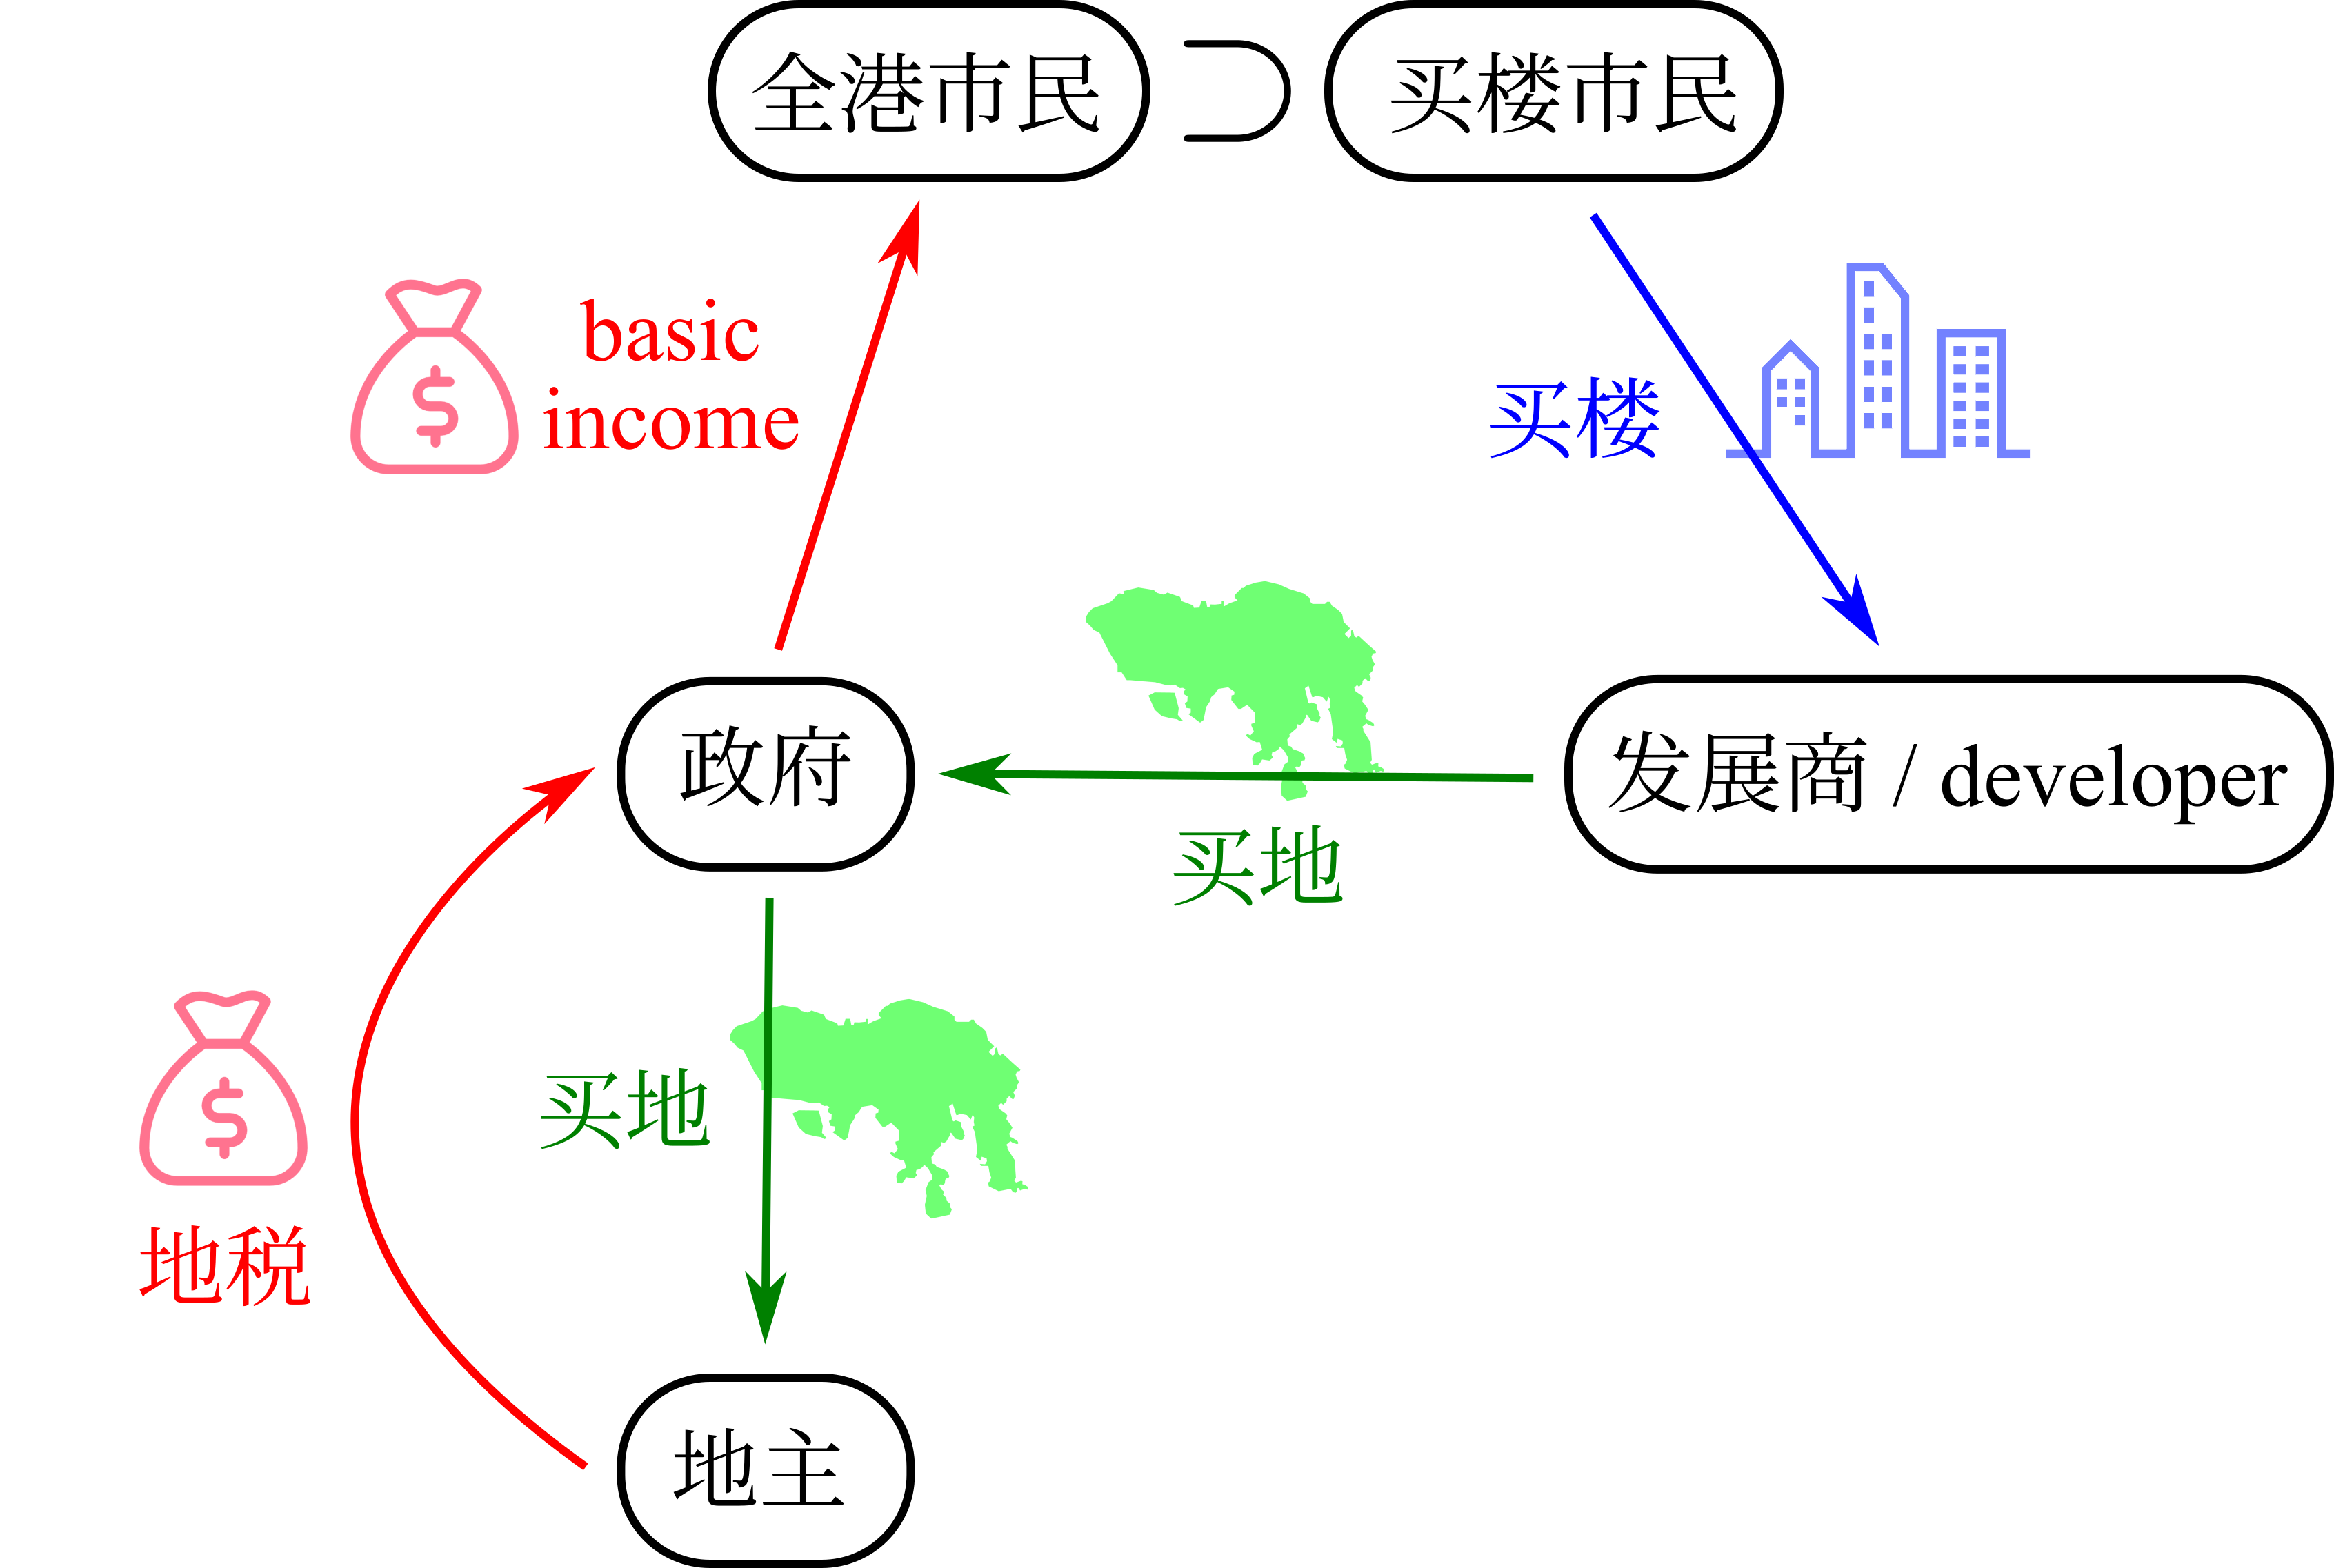
\includegraphics[scale=0.6]{housing-solution.png}}}
\nonumber
\end{equation}
\end{frame}

\frameinlbffalse
\begin{frame}
\frametitle{土地/房屋 问题 (2)}
\begin{itemize}
	\item 在香港进行 \emp{土地改革} 不是没有可能的,但土地的经济学和一般财产可能有不同 \cite{Ryan-Collins2017} \cite{Farvacque-Vitkoviac1992} \cite{Blomley2004} \cite{Linklater2013} \cite{Adams2015},而且涉及「地产霸权」的利益问题: 如果 land tax 仍然不能降低楼价? 

	\item 增加 basic income 的理据

	\item Rent-seeking 不是 land tax 的理由,但稀缺资源是

	\item 如是者,则 land tax 的目的,必然是将稀缺资源作公平分配

	\item 问题是 land tax 要收到什么程度?  也许,直到 平均收入 追得上为止。

	\item 但地税 会 transfer 给租户和住户,导致 楼价 仍然高企。  这样则进一步 增加 basic income.
\end{itemize}
\end{frame}

\frameinlbftrue
\begin{frame}
\frametitle{教育}
\end{frame}

\begin{frame}
\frametitle{医疗}
\end{frame}

\begin{frame}
\frametitle{References}
\printbibliography
\begin{center}
	多谢收看 \smiley
\end{center}
\end{frame}

\end{document} 